%Version 3.1 December 2024
% Flattened (single-file) version of the modular manuscript
% For reviewer consideration — all sections in one file

\documentclass[pdflatex,sn-mathphys-num]{sn-jnl}

%%%% Standard Packages
\usepackage{graphicx}%
\usepackage{multirow}%
\usepackage{amsmath,amssymb,amsfonts}%
\usepackage{amsthm}%
\usepackage{mathrsfs}%
\usepackage[title]{appendix}%
\usepackage{xcolor}%
\usepackage{textcomp}%
\usepackage{manyfoot}%
\usepackage{booktabs}%

\raggedbottom

% !TEX TS-program = pdfLaTeX
% !TeX root=elsarticle-template-harv.tex
%\usepackage{graphicx}
\usepackage{wrapfig}
\usepackage{mathtools} 
%\usepackage{amsthm,amssymb,amsmath}
%\usepackage{comment}
%\usepackage{setspace}
%\usepackage[colorlinks, citecolor=magenta, breaklinks = true]{hyperref}		% for pdflatex
%%\usepackage{caption}
\usepackage{subcaption}
%\usepackage[labelformat=simple]{subcaption}
%\renewcommand\thesubfigure{(\alph{subfigure})}
%\usepackage[ruled,vlined, linesnumbered]{algorithm2e}
%\usepackage{booktabs} 
\usepackage{algorithm}
\usepackage{algorithmic}
\usepackage{arydshln}

\usepackage{tikz}
\usepackage{pgfplots}
\pgfplotsset{compat=1.18} 
%\usepackage{amsthm}
\ifx\theorem\undefined
\newtheorem{theorem}{Theorem}
\fi
%\ifx\proposition\undefined
%\newtheorem{proposition}{Proposition}
%\fi
%\ifx\BlackBox\undefined
%\newcommand{\BlackBox}{\rule{1.5ex}{1.5ex}}  % end of proof
%\fi
%\ifx\proof\undefined
%\newenvironment{proof}{\par\noindent{\em Proof:\ }}{\hfill\BlackBox\\[.0mm]}
%\fi

%%% LOCAL MACRO DEFS
% from b.sty
%\usepackage{amssymb}
%\usepackage{amsmath,amscd}
%\usepackage{amsthm}
%\usepackage{color}
%\usepackage{subfigure}

% Convenient macro for editing, internal notes, etc
\newcommand{\edit}[1]{\textcolor{red}{\textbf{[#1]}}}
\newcommand{\hilite}[1]{\textcolor{red}{#1}}
\newcommand{\note}[1]{\textcolor{blue}{\textbf{\texttt{[#1]}}}}
%\newcommand{\update}[1]{\textcolor{orange}{#1}}
 \newcommand{\update}[1]{#1}
% \newcommand{\note}[1]{\texttt{[#1]}}


% Pretty integrals
% Redefine \int to use integral font from mathabx package
%
% Setup the mathx font (from mathabx.sty)
\DeclareFontFamily{U}{mathx}{\hyphenchar\font45}
\DeclareFontShape{U}{mathx}{m}{n}{
      <5> <6> <7> <8> <9> <10> gen * mathx
      <10.95> mathx10 <12> <14.4> <17.28> <20.74> <24.88> mathx12
      }{}
\DeclareSymbolFont{mathx}{U}{mathx}{m}{n}
\DeclareMathSymbol{\intop}  {1}{mathx}{"B3}

% Independent symbol
\newcommand\independent{\protect\mathpalette{\protect\independenT}{\perp}}
\def\independenT#1#2{\mathrel{\rlap{$#1#2$}\mkern4mu{#1#2}}}

% Horizontal lines
\newcommand{\HRule}[1][0.25mm]{\rule{\linewidth}{#1}}

% Custom bullet for nested lists
\renewcommand{\labelitemii}{$\circ$}

% Shorthand for commonly used tex macros
\newcommand{\wt}{\widetilde}
\newcommand{\wh}{\widehat}
\newcommand{\wb}{\overline}
\newcommand{\cl}{\overline}
\newcommand{\upto}{\nearrow} % increasing
\newcommand{\downto}{\searrow} % decreasing

% Changed Notation
%\newcommand{\vphi}{\phi}
%\renewcommand{\phi}{\varphi} 
%\renewcommand{\varphi}{\vphi}
\let\temp\phi
\let\phi\varphi
\let\varphi\temp
\renewcommand{\Re}{\real}
\renewcommand{\Im}{\imag}
\renewcommand{\sec}{\textsection}
\renewcommand{\S}{\mathbb{S}}
%\renewcommand{\P}{\mathbb{P}}  % replaced by \pr below
\newcommand{\n}{\centernot}         % to simplify negations

% Notation
\newcommand{\pr}{\mathbb{P}}
\newcommand{\C}{\mathbb{C}}
\newcommand{\R}{\mathbb{R}}
\newcommand{\N}{\mathbb{N}}
\newcommand{\Z}{\mathbb{Z}}
\newcommand{\Q}{\mathbb{Q}}
\newcommand{\T}{\mathbb{T}}
\newcommand{\D}{\mathbb{D}}
\newcommand{\E}{\mathbb{E}}
\newcommand{\F}{\mathcal{F}}
\newcommand{\G}{\mathcal{G}}
\newcommand{\normalN}{\mathcal{N}}
\renewcommand{\|}{\,|\,}            % add spacing for conditioning variables
\newcommand{\given}{\,|\,}  % verbose alternative to \|
\newcommand{\Setdef}[2]{\left\{#1 \mid #2\right\} }
\newcommand{\setdef}[2]{\{#1 \mid #2\} }
\newcommand{\fcndef}[3]{#1:#2\rightarrow#3}
\newcommand{\Norm}[1]{\left\Vert#1\right\Vert}
\newcommand{\norm}[1]{\Vert#1\Vert}
\newcommand{\Dotp}[2]{\left\langle#1,#2\right\rangle}
\newcommand{\dotp}[2]{\langle#1,#2\rangle}
\newcommand{\ip}[1]{\langle#1\rangle}
%\newcommand{\br}[1]{\!\left\langle#1\right\rangle\!}
\newcommand{\parder}[2]{\frac{\partial #1}{\partial #2}}
\newcommand{\bd}{\partial}
\newcommand{\eps}{\varepsilon}
%\newcommand{\lap}{\Delta}
\newcommand{\norder}[1]{\parder{#1}{\nu}}
\newcommand{\del}{\nabla}
\newcommand{\grad}{\nabla}
\newcommand{\les}{\lesssim}
\newcommand{\ges}{\gtrsim}
\newcommand{\kldiv}[2]{\KL(#1\,\Vert\,#2)}
\newcommand{\iid}{\overset{\text{iid}}{\sim}}
\newcommand{\symdiff}{\triangle}

% New unary operators
\DeclareMathOperator{\tr}{tr}
\DeclareMathOperator{\supp}{supp}
\DeclareMathOperator{\intr}{int}
\DeclareMathOperator{\diam}{diam}
\DeclareMathOperator{\id}{id}
\DeclareMathOperator{\closure}{cl}
\DeclareMathOperator{\conv}{conv}
\DeclareMathOperator{\vol}{vol}
\DeclareMathOperator{\Div}{div}
\DeclareMathOperator{\sgn}{sgn}
\DeclareMathOperator{\Ric}{Ric}
\DeclareMathOperator{\Cov}{Cov}
\DeclareMathOperator{\Corr}{Corr}
\DeclareMathOperator{\corr}{cor}
\DeclareMathOperator{\cov}{cov}
\DeclareMathOperator{\var}{var}
\DeclareMathOperator{\KL}{KL}
\DeclareMathOperator{\rank}{rank}
\DeclareMathOperator{\Span}{span}
\DeclareMathOperator{\Null}{null} % \null already defined
\DeclareMathOperator{\real}{Re}
\DeclareMathOperator{\imag}{Im}
\DeclareMathOperator{\diag}{diag}
\DeclareMathOperator{\ran}{ran}
\DeclareMathOperator{\dom}{dom}
%\DeclareMathOperator{\argmin}{arg\,min}
\DeclareMathOperator*{\argmin}{arg\,min}
%\DeclareMathOperator{\argmax}{arg\,max}
\DeclareMathOperator*{\argmax}{arg\,max}
\DeclareMathOperator{\dist}{dist}
\DeclareMathOperator\ext{ext}

% Probability distributions
\DeclareMathOperator{\PoissonDist}{Poisson}
\DeclareMathOperator{\BernoulliDist}{Ber}
\DeclareMathOperator{\GammaDist}{Gamma}
\DeclareMathOperator{\ExpDist}{Exp}
\DeclareMathOperator{\NormalDist}{Normal}
\DeclareMathOperator{\NegbinomDist}{NegBinom}
\DeclareMathOperator{\UniformDist}{Unif}
\DeclareMathOperator{\GumbelDist}{Gumbel}

%\usepackage{microtype}
%\usepackage{graphicx}
%\usepackage{booktabs}
%%\usepackage{algorithm}
%
%\newcommand{\description}{}
\usepackage{enumitem}
%\usepackage{pgfplots}
%\usepackage{subcaption}
%\usepackage{cleveref}
%
%% Convenient macro for editing, internal notes, etc
%\usepackage{color}
%\usepackage{enumitem}
%
\newcommand{\dagspace}{\mathbb{D}} %{\mathsf{DAG}}
\newcommand{\wadj}{\R^{d\times d}}
\newcommand{\bin}{\{0,1\}^{d\times d}}
\newcommand{\dags}{\mathbb{D}}
\newcommand{\adj}{\mathcal{A}}
% \newcommand{\atoms}{\mathcal{A}}
\newcommand{\perms}{\mathbb{S}}
\newcommand{\lowers}{\mathcal{L}}
\newcommand{\ecp}{\mathsf{ECP}}
\newcommand{\spec}{r}

\newcommand{\Gauss}{\mathsf{Gauss}}
\newcommand{\Exp}{\mathsf{Exp}}
\newcommand{\Gumbel}{\mathsf{Gumbel}}
\newcommand{\Logistic}{\mathsf{Logistic}}

\newcommand{\FGS}{\text{FGS}}
\newcommand{\fgsest}{B_{\FGS}}

\newcommand{\dat}{\mathbf{X}}

\newcommand{\method}{\text{NOTEARS}}
\newcommand{\methodreg}{\text{NOTEARS-}\ell_{1}}
\newcommand{\true}{W}
\newcommand{\truecol}{w}
\newcommand{\trueadj}{B}
\newcommand{\est}{\widehat{W}}
\newcommand{\adjest}{\widehat{B}}
\newcommand{\estecp}{\widetilde{W}_{\ecp}}
\newcommand{\estgob}{W_{\gr}}

\newcommand{\loss}{\ell}
\newcommand{\scoregr}{Q}
\newcommand{\score}{F}
\newcommand{\gr}{\mathsf{G}}
\newcommand{\ver}{\mathsf{V}}
\newcommand{\edg}{\mathsf{E}}
\DeclareMathOperator{\pa}{pa}
\newcommand{\hess}{\nabla^{2}}
\DeclareMathOperator{\vect}{vec}


%\theoremstyle{plain}
%\newtheorem{theorem}{Theorem}[section]
%\newtheorem{lemma}[theorem]{Lemma}
%\newtheorem{proposition}[theorem]{Proposition}
%\newtheorem{corollary}[theorem]{Corollary}
%
%\theoremstyle{definition}
%\newtheorem{definition}{Definition}[section]
%\newtheorem{conj}{Conjecture}[section]
%\newtheorem{exmp}{Example}[section]
\numberwithin{equation}{section}



\begin{document}

\title[Graph Structure Learning for Traffic Prediction]{Graph Structure Learning for Traffic Prediction}

\author*[1]{\fnm{Mahmood} \sur{Amintoosi}}\email{m.amintoosi@um.ac.ir}

\affil*[1]{\orgdiv{Division of Computer Science, Department of Applied Mathematics, Faculty of Mathematical Sciences}, \orgname{Ferdowsi University of Mashhad}, \orgaddress{\street{Bahonar Av.}, \city{Mashhad}, \postcode{91775}, \state{Khorasan-e Razavi}, \country{IRAN}}, ORCID:0000-0001-9640-6475}

\begin{abstract}
Graph-based traffic forecasting methods typically rely on predefined adjacency matrices derived from physical road proximity. However, dense physical connectivity can induce excessive spatial aggregation---a form of oversmoothing---that degrades prediction accuracy. We propose a multi-lag graph structure learning framework that discovers temporally heterogeneous functional dependencies between traffic sensors. Using DAGMA continuous optimization, we construct lag-specific dependency graphs from explicit temporal input blockings of the form $Z = [x(t{-}L), \ldots, x(t)]$, yielding separate functional graphs for each temporal lag. A GatedMultiGraphTGCN architecture then adaptively selects among these lag-specific graphs through a per-node, per-timestep learned gate. Experiments on the Los-loop highway dataset demonstrate a mean RMSE improvement of 14.9\% over a no-graph baseline across five random seeds, with the improvement robust to a parameter-matched control. A lag ablation study confirms that all three temporal lags contribute complementary information. On the SZ-Taxi urban dataset, improvements are marginal, indicating dataset dependence. These findings establish that temporally heterogeneous graph structures can substantially benefit traffic forecasting when the underlying dependency patterns vary across temporal scales.
\end{abstract}
\keywords{
Traffic Forecasting,
Graph Structure Learning,
Multi-Lag Dependency Learning,
Graph Convolutional Networks,
Adaptive Graph Gating
}
\maketitle

% ============================================================
% SECTION: introduction
% ============================================================

\section{Introduction}\label{sec:introduction}

Traffic prediction is a fundamental challenge in intelligent transportation systems, requiring models that capture complex spatial and temporal dependencies in urban road networks \citep{akhtar2021review}. Graph Convolutional Networks (GCNs) \citep{kipf2017semi} and Temporal GCNs (T-GCNs) \citep{zhao2019t} have emerged as effective approaches by modeling traffic networks as graphs, where nodes represent road segments and edges encode spatial relationships.

A critical limitation of existing graph-based methods is their reliance on predefined adjacency matrices derived from physical road proximity \citep{zhao2019t}. A systematic bibliometric analysis of 784 traffic forecasting articles (2000--2025) confirms that graph-based methods now dominate the field, yet nearly all depend on heuristic graph construction from road network topology (see Appendix~\ref{sec:Bibliometric-Methodology}). However, physical connectivity is an imperfect proxy for functional traffic dependency: roads that are physically distant may exhibit strong traffic correlations due to commuting patterns, while adjacent roads may have minimal mutual influence \citep{Chen2022}.

A second, less recognized problem is that dense physical graphs can induce \textit{oversmoothing} in GCN-based models. When the adjacency matrix encodes hundreds or thousands of edges, repeated graph convolution operations aggregate information from increasingly distant nodes, causing node representations to converge and lose discriminative power. This excessive spatial aggregation can paradoxically degrade forecasting performance compared to using no graph at all.

Graph Structure Learning (GSL) addresses the first problem by learning the adjacency matrix directly from traffic data rather than relying on physical proximity. Recent work has applied continuous DAG optimization methods such as NOTEARS \citep{zheng2018dags} and DAGMA \citep{Bello2024DAGMA} to this task, discovering sparse functional dependencies that differ substantially from physical road connectivity \citep{Amintoosi1403aimc55-GSL}.

However, a single static learned graph has an inherent limitation: traffic dependencies are \textit{temporally heterogeneous}. The influence of sensor $i$ on sensor $j$ may vary depending on the temporal lag---a 5-minute delay captures different traffic propagation patterns than a 15-minute delay. A single adjacency matrix cannot represent these lag-specific structures.

In this paper, we address this limitation through two contributions:

\begin{enumerate}
    \item \textbf{Multi-lag DAGMA:} We construct explicit temporal input blockings $Z = [x(t{-}L), \ldots, x(t)]$ and apply DAGMA to learn a weight matrix whose blocks correspond to lag-specific temporal functional dependencies. This provides direct, interpretable evidence for which temporal lags carry predictive information.

    \item \textbf{GatedMultiGraphTGCN:} We propose a T-GCN variant that processes each lag-specific graph separately and uses a per-node, per-timestep learned gate to adaptively combine the resulting representations.
\end{enumerate}

Experiments on the Los-loop highway dataset demonstrate that GatedMultiGraphTGCN achieves a mean RMSE improvement of 14.9\% over a no-graph baseline, validated across five random seeds and confirmed against a parameter-matched control. A lag ablation study shows that all three temporal lags contribute complementary information. On the SZ-Taxi urban dataset, improvements are marginal, and we explicitly report this dataset dependence rather than claiming universal benefit.

The remainder of this paper is organized as follows. Section~\ref{sec:bg} reviews background on GCNs and T-GCNs. Section~\ref{sec:method} presents the multi-lag DAGMA formulation and GatedMultiGraphTGCN architecture. Section~\ref{sec:experiments} describes the experimental setup. Section~\ref{sec:results} presents results. Section~\ref{sec:discussion} discusses findings. Section~\ref{sec:limitations} states limitations. Section~\ref{sec:conclusion} concludes.

% ============================================================
% SECTION: background
% ============================================================

\section{Background}\label{sec:bg}

\subsection{Problem Formulation}

We model the road network as a graph $G=(V,E)$, where $V=\{v_1,\ldots,v_N\}$ represents $N$ road segments and $\mathbf{A} \in \{0,1\}^{N \times N}$ is the binary adjacency matrix encoding road connectivity. Traffic data is represented by a feature matrix $X \in \mathbb{R}^{T \times N}$, where $X_t \in \mathbb{R}^N$ represents traffic speeds across all roads at time $t$. The forecasting task learns a mapping from historical observations to future traffic conditions:
\begin{equation}
[X_{t+1},\ldots,X_{t+T}] = f(G;[X_{t-n},\ldots,X_t])
\end{equation}
where $n$ is the historical window size and $T$ is the prediction horizon.

\subsection{Graph Convolutional Networks}

GCNs extend convolution to graph-structured data through a layer-wise propagation rule \citep{kipf2017semi}:
\begin{equation}
\mathbf{H}^{(l+1)}= \sigma\!\left(\tilde{\mathbf{D}}^{-\frac{1}{2}} \tilde{\mathbf{A}}\tilde{\mathbf{D}}^{-\frac{1}{2}}\mathbf{H}^{(l)} \mathbf{W}^{(l)} \right)
\label{eq:gcn-layer}
\end{equation}
where $\tilde{\mathbf{A}} = \mathbf{A} + \mathbf{I}_N$ is the adjacency matrix with self-connections, $\tilde{\mathbf{D}}$ is the degree matrix, $\mathbf{W}^{(l)}$ is a trainable weight matrix, and $\sigma(\cdot)$ is a nonlinear activation. The normalized adjacency $\hat{A}=\tilde{\mathbf{D}}^{-\frac{1}{2}} \tilde{\mathbf{A}}\tilde{\mathbf{D}}^{-\frac{1}{2}}$ aggregates information from neighboring nodes while preserving feature scale. A two-layer GCN is:
\begin{equation}
f(\mathbf{A},\mathbf{X})=\sigma\!\left(\hat{A}\sigma\!\left(\hat{A}\mathbf{X} \mathbf{W}^{(1)} \right) \mathbf{W}^{(2)} \right)
\label{eq:two-layer-gcn}
\end{equation}

\subsection{Temporal Graph Convolutional Network}

The T-GCN \citep{zhao2019t} combines GCN for spatial feature extraction with a Gated Recurrent Unit (GRU) for temporal modeling. At each timestep, the GCN extracts spatial features $\mathbf{Z}_t=f(\mathbf{A},\mathbf{X}_t)$, which are then processed by the GRU to capture temporal dynamics. The GRU uses update gate $\mathbf{u}_t$, reset gate $\mathbf{r}_t$, and candidate hidden state $\mathbf{c}_t$ with learnable weight matrices $\mathbf{W}_u$, $\mathbf{W}_r$, $\mathbf{W}_c$. The model is trained by minimizing:
\begin{equation}
\mathcal{L}=\| Y_{t}-\widehat{Y_{t}}\|_2+\lambda \|\Theta\|_1
\end{equation}
where $\widehat{Y_{t}}$ is the prediction, $Y_t$ is the ground truth, and $\lambda$ controls L1 regularization.

% ============================================================
% SECTION: method
% ============================================================

\section{Proposed Method}\label{sec:method}

\subsection{Motivation for Data-Driven Graph Structure Learning}

In both GCN \citep{kipf2017semi} and T-GCN \citep{zhao2019t}, the adjacency matrix $\mathbf{A}$ is predefined based on physical road proximity. This has two fundamental limitations. First, physical connectivity is an imperfect proxy for functional traffic dependency: roads that are physically distant may exhibit strong traffic correlations due to commuting patterns, while adjacent roads may have minimal mutual influence. Second, dense physical graphs (e.g., 2833 edges for 207 nodes in the Los-loop dataset) can induce oversmoothing through excessive spatial aggregation in graph convolution layers.

Graph Structure Learning addresses these limitations by learning $\mathbf{A}$ directly from traffic data. We employ DAGMA \citep{Bello2024DAGMA}, which extends the NOTEARS framework \citep{zheng2018dags} for continuous DAG optimization.

\subsection{DAGMA-Based Graph Structure Learning}

DAGMA models the data through a structural equation model defined by a weighted adjacency matrix $W \in \mathbb{R}^{d \times d}$. Instead of operating on the discrete space of DAGs, it optimizes over continuous real matrices with a smooth acyclicity constraint $h(W) = 0$, where:
\begin{equation}
h(W) = \tr\big(e^{W \circ W}\big) - d = 0
\end{equation}
and $\circ$ denotes the Hadamard product. The optimization uses an augmented Lagrangian:
\begin{equation}
L^\rho(W, \alpha) = \text{score}(W) + \frac{\rho}{2}|h(W)|^2 + \alpha h(W)
\end{equation}
where $\text{score}(W)$ measures data fit, $\alpha$ is the Lagrange multiplier, and $\rho > 0$ is a penalty parameter. The algorithm iteratively updates $W$ until $h(W) < \epsilon$, then applies thresholding: $\hat{W} = W \circ \mathbf{1}(|W| > \omega)$.

\textbf{Convention:} Throughout this paper, we follow the DAGMA convention where $W[i,j]$ represents a directed dependency from variable $i$ to variable $j$.

\subsection{Multi-Lag DAGMA Formulation}\label{sec:multilag}

A single learned graph captures contemporaneous or aggregated dependencies but cannot distinguish between different temporal scales of traffic propagation. To address this, we construct an explicit multi-lag input representation.

Given traffic observations $x(t) \in \mathbb{R}^N$ and a lag window $L$, we define the multi-lag input:
\begin{equation}
Z_t = \big[x(t{-}L),\; x(t{-}L{+}1),\; \ldots,\; x(t{-}1),\; x(t)\big] \in \mathbb{R}^{(L+1) \times N}
\end{equation}
which is flattened to a vector of dimension $(L+1) \cdot N$. The matrix $Z$ is formed by stacking $Z_t$ over all training time steps.

Applying DAGMA to $Z$ produces a weight matrix $W \in \mathbb{R}^{(L+1)N \times (L+1)N}$. The block structure of $W$ is:
\begin{itemize}
    \item $W[l \cdot N : (l{+}1) \cdot N,\; L \cdot N : (L{+}1) \cdot N]$ represents dependencies from lag $l$ to the current time step
    \item $W[L \cdot N : (L{+}1) \cdot N,\; L \cdot N : (L{+}1) \cdot N]$ represents contemporaneous dependencies
\end{itemize}

Since $W[i,j]$ means variable $i \rightarrow$ variable $j$, the block $W[l \cdot N + i,\; L \cdot N + j]$ captures the functional dependency from sensor $i$ at time $t{-}(L{-}l)$ to sensor $j$ at time $t$. This provides explicit, interpretable lag-specific temporal functional dependencies.

For each lag $l$, we extract the corresponding block and apply thresholding and self-loop removal to obtain a binary adjacency matrix:
\begin{equation}
A_l[i,j] = \mathbf{1}\big(|W[l \cdot N + i,\; L \cdot N + j]| > \tau\big) \cdot (1 - \delta_{ij})
\end{equation}
where $\tau$ is a threshold and $\delta_{ij}$ is the Kronecker delta.

For $L=3$, this yields four blocks: lag$_3$ ($x(t{-}3) \rightarrow x(t)$), lag$_2$ ($x(t{-}2) \rightarrow x(t)$), lag$_1$ ($x(t{-}1) \rightarrow x(t)$), and current ($x(t) \rightarrow x(t)$). Empirically, these blocks exhibit substantially different edge structures with low cross-lag overlap, confirming that traffic dependencies are temporally heterogeneous.

\subsection{GatedMultiGraphTGCN}\label{sec:gatedmulti}

Standard T-GCN uses a single adjacency matrix for all timesteps. We propose GatedMultiGraphTGCN, which processes each lag-specific graph separately and adaptively combines the results.

\subsubsection{Architecture}

Given $K$ lag-specific graphs $\{A_1, \ldots, A_K\}$, we precompute their graph Laplacians $\{L_1, \ldots, L_K\}$. At each input timestep $t$:

\begin{enumerate}
    \item The gate network computes per-node, per-graph weights:
    \begin{equation}
    \alpha_t = \text{softmax}\big(\text{MLP}([x_t; h_{t-1}])\big) \in \mathbb{R}^{N \times K}
    \end{equation}
    where $[x_t; h_{t-1}]$ concatenates the current input and previous hidden state.

    \item A weighted adjacency is formed:
    \begin{equation}
    \tilde{L}_t = \sum_{k=1}^{K} \alpha_t^{(k)} \cdot L_k \in \mathbb{R}^{N \times N}
    \end{equation}

    \item Graph convolution uses this adaptive adjacency:
    \begin{equation}
    g_t = \tilde{L}_t \cdot [x_t; h_{t-1}]
    \end{equation}

    \item The GRU update proceeds with $g_t$:
    \begin{align}
    z_t &= \sigma(W_z \cdot g_t) \\
    r_t, u_t &= \text{chunk}(z_t) \\
    c_t &= \tanh(W_n \cdot [x_t; r_t \odot h_{t-1}]) \\
    h_t &= u_t \odot h_{t-1} + (1 - u_t) \odot c_t
    \end{align}
\end{enumerate}

\subsubsection{Key Properties}

The gate operates at three levels simultaneously:
\begin{itemize}
    \item \textbf{Per-node:} each of the $N$ nodes has independent gate weights, allowing different sensors to use different lag graphs
    \item \textbf{Per-timestep:} the gate recomputes at each of the 12 input steps, adapting to the temporal context
    \item \textbf{Differentiable:} the gate is learned jointly with the forecasting objective via backpropagation
\end{itemize}

This contrasts with simpler multi-graph approaches:
\begin{itemize}
    \item \textbf{UnionGraph:} merges all lag graphs into one adjacency, losing lag-specific information
    \item \textbf{WeightedMulti:} learns a fixed global weight per lag graph, without per-node or per-timestep adaptation
    \item \textbf{MultiGraph:} assigns graphs to timesteps in a fixed cyclic pattern
\end{itemize}

\subsubsection{Parameter Count}

For hidden dimension $H$ and $K$ lag graphs, GatedMultiGraphTGCN has approximately $3H^2 + 6H + (H+1)H + H + (H+1)K + K$ parameters. With $H=64$ and $K=3$, this yields 17,091 parameters, compared to 12,672 for standard T-GCN. A parameter-matched control (Section~\ref{sec:param_control}) confirms that this capacity difference does not explain the performance improvement.

% ============================================================
% SECTION: experiments
% ============================================================

\section{Experimental Setup}\label{sec:experiments}

\subsection{Datasets}

We evaluate on two widely-used traffic datasets:

\begin{itemize}
    \item \textbf{SZ-Taxi:} Taxi trajectory data from Shenzhen, China (January 2015), with speed measurements from 156 sensors aggregated at 15-minute intervals. The physical graph has 532 edges.
    \item \textbf{Los-loop:} Real-time traffic speed data from 207 loop detectors on Los Angeles County highways (March 1--7, 2012), aggregated every 5 minutes. The physical graph has 2833 edges.
\end{itemize}

Both datasets are split into training (80\%) and testing (20\%) sets, preserving temporal order. Performance is evaluated across prediction horizons PH $\in \{1, 2, 3, 4\}$.

\subsection{Multi-Lag DAGMA Configuration}

For the multi-lag formulation, we use lag window $L=3$, yielding input dimension $(L+1) \cdot N$:
\begin{itemize}
    \item SZ-Taxi: $4 \times 156 = 624$ variables
    \item Los-loop: $4 \times 207 = 828$ variables
\end{itemize}

DAGMA hyperparameters: $\lambda_1 = 0.01$, loss type = L2, warm-up iterations = 30,000, max iterations = 60,000. The DAGMA output is thresholded at $\tau = 0.1$ and self-loops are removed. DAGMA is applied only to training data; test data never enters the graph construction.

\subsection{Forecasting Models}

We compare the following T-GCN variants:

\begin{itemize}
    \item \textbf{NoGraph:} T-GCN with identity adjacency (no spatial information). This is the critical baseline---it tests whether any graph helps.
    \item \textbf{Physical:} T-GCN with the predefined road network adjacency.
    \item \textbf{MultiGraph\_fixed:} T-GCN that assigns lag-specific graphs to input timesteps in a fixed pattern (corrected alignment).
    \item \textbf{GatedMultiGraphTGCN:} Our proposed method with adaptive per-node, per-timestep gating over lag-specific graphs.
\end{itemize}

All models use hidden dimension $H=64$, Adam optimizer (learning rate 0.001, weight decay 0.0001), batch size 128, historical window $n=12$, and 50 training epochs. The loss function is MSE with L1 regularization. Results are reported as mean $\pm$ standard deviation over 5 random seeds (seeds 42--46) for the main comparison.

\subsection{Evaluation Metrics}

We report Root Mean Squared Error (RMSE) and Mean Absolute Error (MAE):
\begin{equation}
\text{RMSE} = \sqrt{\frac{1}{n}\sum_{i=1}^{n}(Y_i - \hat{Y}_i)^2}, \quad
\text{MAE} = \frac{1}{n}\sum_{i=1}^{n}|Y_i - \hat{Y}_i|
\end{equation}
where $Y_i$ and $\hat{Y}_i$ are actual and predicted traffic speeds. RMSE is the primary metric.

% ============================================================
% SECTION: results
% ============================================================

\section{Results}\label{sec:results}

\subsection{Dense Physical Graphs and Oversmoothing}\label{sec:oversmoothing}

A fundamental finding across our experiments is that dense physical graphs degrade T-GCN performance. Table~\ref{tab:oversmoothing} compares the physical graph against a no-graph baseline and sparse learned graphs.

\begin{table}[t]
\centering
\caption{Oversmoothing evidence: Los-loop (PH=1, seed=42). Dense physical graphs produce substantially worse RMSE than no graph at all. Sparse learned graphs and multi-lag graphs improve over NoGraph.}
\label{tab:oversmoothing}
\begin{tabular}{lccc}
\toprule
\textbf{Graph} & \textbf{Edges} & \textbf{RMSE} & \textbf{MAE} \\
\midrule
Physical (207 nodes) & 2833 & 7.658 & 5.329 \\
NoGraph (identity) & 207 & 5.143 & 3.028 \\
Single DAGMA ($\tau$=0.3) & 6 & 5.213 & 3.192 \\
Single DAGMA ($\tau$=0.1) & 60 & 6.057 & 3.693 \\
MultiGraph\_fixed & 30 & 4.715 & 2.755 \\
GatedMultiGraphTGCN & 30 & 4.458 & 2.696 \\
\bottomrule
\end{tabular}
\end{table}

The physical graph (2833 edges) produces RMSE of 7.658, while NoGraph (identity adjacency) achieves 5.143---a 32.8\% improvement from removing the graph entirely. This confirms that dense spatial aggregation hurts forecasting. The sparse MultiGraph and GatedMulti approaches further improve over NoGraph, demonstrating that carefully structured sparse graphs can provide genuine benefit.

\subsection{Multi-Lag Graph Structure}\label{sec:multilag_structure}

The multi-lag DAGMA formulation ($L=3$) produces lag-specific graphs with substantially different structures. Table~\ref{tab:lag_stats} reports the statistics for Los-loop at threshold $\tau = 0.1$.

\begin{table}[t]
\centering
\caption{Multi-lag DAGMA block statistics (Los-loop, $L=3$, $\tau=0.1$). Different lag blocks capture different dependency structures.}
\label{tab:lag_stats}
\begin{tabular}{lcccc}
\toprule
\textbf{Block} & \textbf{Interpretation} & \textbf{Edges} & \textbf{Max $|w|$} & \textbf{Density} \\
\midrule
current & $x(t) \rightarrow x(t)$ & 70 & 0.653 & 0.001634 \\
lag\_1 & $x(t{-}1) \rightarrow x(t)$ & 90 & 0.804 & 0.002100 \\
lag\_2 & $x(t{-}2) \rightarrow x(t)$ & 5 & 0.673 & 0.000117 \\
lag\_3 & $x(t{-}3) \rightarrow x(t)$ & 16 & 0.296 & 0.000373 \\
\bottomrule
\end{tabular}
\end{table}

The current block has 70 cross-sensor edges, lag\_1 has 90 edges (dominated by self-loops), lag\_2 has only 5 edges, and lag\_3 has 16 edges. These blocks are structurally distinct, confirming that traffic dependencies are temporally heterogeneous.

\subsection{Multi-Seed Validation}\label{sec:multiseed}

Table~\ref{tab:multiseed} presents the primary result: Los-loop, PH=1, five random seeds.

\begin{table}[t]
\centering
\caption{Multi-seed validation on Los-loop (PH=1). GatedMultiGraphTGCN outperforms NoGraph in all five seeds. Mean improvement: 14.9\%.}
\label{tab:multiseed}
\begin{tabular}{lcccccc}
\toprule
\textbf{Method} & \textbf{S42} & \textbf{S43} & \textbf{S44} & \textbf{S45} & \textbf{S46} & \textbf{Mean$\pm$Std} \\
\midrule
NoGraph & 5.143 & 5.281 & 5.386 & 5.205 & 5.154 & 5.234$\pm$0.090 \\
MultiGraph\_fixed & 4.717 & 4.737 & 4.752 & 4.994 & 4.771 & 4.794$\pm$0.102 \\
\textbf{GatedMulti} & \textbf{4.458} & \textbf{4.660} & \textbf{4.335} & \textbf{4.261} & \textbf{4.547} & \textbf{4.452$\pm$0.143} \\
\bottomrule
\end{tabular}
\end{table}

GatedMultiGraphTGCN beats NoGraph in all 5 seeds with a mean RMSE of 4.452 versus 5.234, corresponding to a 14.9\% improvement. The fixed multi-graph approach also consistently outperforms NoGraph (8.4\% improvement), but GatedMulti provides an additional 7.1\% improvement through adaptive gating.

\subsection{Parameter-Matched Control}\label{sec:param_control}

To rule out the explanation that GatedMulti's improvement comes from having more parameters, we compare against a NoGraph T-GCN with matched capacity (Table~\ref{tab:param_control}).

\begin{table}[t]
\centering
\caption{Parameter-matched control (Los-loop, PH=1, seed=42). Adding 35\% more parameters to NoGraph improves RMSE by only 0.1\%. GatedMulti's improvement is from the gating architecture.}
\label{tab:param_control}
\begin{tabular}{lccc}
\toprule
\textbf{Model} & \textbf{hidden\_dim} & \textbf{Parameters} & \textbf{RMSE} \\
\midrule
NoGraph & 64 & 12,672 & 5.143 \\
NoGraph (larger) & 74 & 16,872 & 5.137 \\
\textbf{GatedMulti} & 64 & \textbf{17,091} & \textbf{4.458} \\
\bottomrule
\end{tabular}
\end{table}

The parameter-matched NoGraph (16,872 parameters) achieves RMSE 5.137, virtually identical to the standard NoGraph (5.143). GatedMulti (17,091 parameters) achieves 4.458. Thus 99\% of the improvement comes from the gating architecture, not from additional capacity.

\subsection{Lag Ablation}\label{sec:lag_ablation}

Table~\ref{tab:lag_ablation} shows the contribution of each temporal lag.

\begin{table}[t]
\centering
\caption{Lag ablation (Los-loop, PH=1, seed=42). All three lags contribute; the full combination is best.}
\label{tab:lag_ablation}
\begin{tabular}{lccc}
\toprule
\textbf{Configuration} & \textbf{Edges} & \textbf{RMSE} & \textbf{Improvement} \\
\midrule
NoGraph & 207 & 5.143 & --- \\
lag\_2 only & 3 & 4.619 & 10.2\% \\
lag\_3 only & 15 & 4.605 & 10.5\% \\
lag\_1 only & 12 & 4.605 & 10.5\% \\
lag\_1+lag\_3 & 27 & 4.646 & 9.7\% \\
lag\_2+lag\_3 & 18 & 4.638 & 9.8\% \\
lag\_1+lag\_2 & 15 & 4.559 & 11.4\% \\
\textbf{All 3 lags} & \textbf{30} & \textbf{4.458} & \textbf{13.3\%} \\
\bottomrule
\end{tabular}
\end{table}

Each individual lag provides approximately 10\% improvement over NoGraph. The best two-lag combination is lag\_1+lag\_2 (11.4\%), and the full three-lag configuration achieves 13.3\%. This confirms that all three temporal scales carry complementary predictive information.

\subsection{Prediction Horizons and Dataset Dependence}\label{sec:multiph}

Table~\ref{tab:multiph} reports results across all four prediction horizons.

\begin{table}[t]
\centering
\caption{Multi-horizon results on Los-loop (seed=42). GatedMulti consistently outperforms NoGraph and Physical across all horizons.}
\label{tab:multiph}
\begin{tabular}{lcccc}
\toprule
\textbf{Method} & \textbf{PH=1} & \textbf{PH=2} & \textbf{PH=3} & \textbf{PH=4} \\
\midrule
Physical & 7.658 & 8.002 & 8.512 & 8.540 \\
NoGraph & 5.143 & 5.642 & 6.164 & 6.502 \\
MultiGraph\_fixed & 4.715 & 5.549 & 5.934 & 6.336 \\
\textbf{GatedMulti} & \textbf{4.458} & \textbf{5.308} & \textbf{5.687} & \textbf{6.004} \\
\bottomrule
\end{tabular}
\end{table}

GatedMulti consistently outperforms NoGraph across all horizons, with the largest relative improvement at PH=1 (13.3\%). The advantage persists but narrows at longer horizons.

\textbf{Dataset dependence.} On SZ-Taxi, GatedMulti shows only marginal improvement over NoGraph (PH=1: 4.108 vs.\ 4.116; PH=4: 4.221 vs.\ 4.221). This dataset dependence is an important finding: the multi-lag approach is most effective when the underlying traffic network exhibits strong lag-specific dependencies, as appears to be the case for the Los-loop highway network.

\subsection{Relation to Original GSL/cGSL Results}

The original GSL/cGSL experiments (see Appendix~\ref{app:original_gsl}) established that replacing physical adjacency with DAGMA-learned graphs improves GCN and T-GCN performance, with different optimal graph structures for each backbone (cyclic for GCN, acyclic for T-GCN). These findings motivated the deeper investigation into temporal dependency structure that led to the multi-lag formulation. The multi-lag approach represents a methodological advance over the single-graph GSL: instead of learning one graph and debating its interpretation, we explicitly construct lag-specific graphs and let the model decide how to use them.

% ============================================================
% SECTION: discussion
% ============================================================

\section{Discussion}\label{sec:discussion}

\subsection{Why Dense Physical Graphs Fail}

The most striking finding is that removing the physical graph entirely improves RMSE by 32.8\% (Table~\ref{tab:oversmoothing}). This oversmoothing effect arises because the physical graph's high density (2833 edges for 207 nodes) causes repeated graph convolution operations to aggregate information from increasingly distant and irrelevant nodes, washing out the distinctive features of individual road segments. This finding is consistent across both datasets and aligns with theoretical predictions about over-squashing in graph neural networks.

\subsection{Why Multi-Lag Processing Helps}

The multi-lag formulation provides two distinct advantages. First, it makes the temporal dependency structure explicit: instead of learning a single ambiguous graph, we obtain separate graphs for each temporal lag, each with a clear interpretation (Table~\ref{tab:lag_stats}). Second, the GatedMultiGraphTGCN architecture can process these graphs through separate T-GCN cells and adaptively combine the results, preserving the lag-specific information that would be lost by merging into a single adjacency.

The fact that MultiGraph\_fixed (same edges, fixed assignment) achieves 4.794 while GatedMulti achieves 4.452 demonstrates that \textit{how} the lag-specific graphs are processed matters as much as \textit{which} graphs are used. The 0.342 RMSE improvement from adaptive gating represents a 7.1\% further reduction beyond the fixed multi-graph approach.

\subsection{Why the Effect is Dataset-Dependent}

The marginal improvement on SZ-Taxi (0.2--0.9\%) compared to the strong improvement on Los-loop (14.9\%) likely reflects differences in the underlying traffic dynamics. The Los-loop dataset captures highway traffic where propagation patterns have clear temporal structure (vehicles traveling at highway speeds create predictable lagged dependencies). The SZ-Taxi dataset captures urban taxi traffic, which may have more complex, less structured dependencies that are not well captured by fixed-lag analysis. This dataset dependence is an honest finding that the paper explicitly reports rather than hiding.

\subsection{Connection to Original GSL/cGSL Findings}

The original GSL/cGSL experiments established that learned sparse graphs outperform dense physical graphs, and that different backbone architectures (GCN vs T-GCN) benefit from different graph structures. These findings remain valid and motivated the deeper investigation into temporal heterogeneity. The multi-lag formulation can be viewed as a principled extension: rather than debating whether the learned graph should be cyclic or acyclic, we construct lag-specific graphs that naturally capture different temporal aspects of the dependency structure.

% ============================================================
% SECTION: limitations
% ============================================================

\section{Limitations}\label{sec:limitations}

This study has several limitations that delineate the boundaries of the current evidence:

\begin{enumerate}
    \item \textbf{Dataset dependence:} The strong improvement (14.9\%) is observed on the Los-loop highway dataset, while the SZ-Taxi urban dataset shows only marginal improvement. The method's effectiveness appears to depend on the underlying traffic dynamics.

    \item \textbf{Two datasets only:} Evaluation is limited to two traffic datasets. Broader validation on diverse traffic networks (e.g., different cities, different sensor types, different time periods) would strengthen generalizability claims.

    \item \textbf{DAGMA scalability:} The multi-lag formulation increases the DAGMA input dimension to $(L+1) \cdot N$. For the Los-loop dataset ($N=207$), this yields an $828 \times 828$ matrix requiring approximately 4 hours of computation. Scaling to networks with thousands of sensors would require more efficient graph learning algorithms.

    \item \textbf{Fixed lag window:} The current formulation uses a fixed lag window $L=3$. The optimal lag structure may vary across datasets and traffic conditions. Adaptive lag selection remains future work.

    \item \textbf{Static learned graphs:} The lag-specific graphs are learned once from training data and remain fixed during inference. While the GRU hidden state provides temporal dynamics and the gate provides per-timestep graph selection, the underlying dependency graphs themselves do not adapt to changing traffic conditions.

    \item \textbf{Limited backbone architectures:} We evaluate only T-GCN as the backbone. Whether the multi-lag approach benefits other graph-based forecasting architectures (e.g., ST-GCN, Graph WaveNet) remains to be tested.

    \item \textbf{No causal identification:} The DAGMA formulation discovers temporal functional dependencies, not causal relationships. We do not claim that the learned graphs represent causal traffic mechanisms.

    \item \textbf{Prediction horizons:} Results are reported for horizons PH=1--4. The method's behavior at longer horizons (e.g., 30--60 minutes) is not evaluated.
\end{enumerate}

% ============================================================
% SECTION: conclusion
% ============================================================

\section{Conclusion}\label{sec:conclusion}

This paper addresses two fundamental challenges in graph-based traffic forecasting: the oversmoothing caused by dense physical graphs, and the temporal heterogeneity of traffic dependencies that a single static graph cannot capture.

Our key findings are:

\begin{enumerate}
    \item Dense physical road-network graphs can severely degrade GCN/T-GCN forecasting performance through excessive spatial aggregation. On the Los-loop dataset, removing the physical graph entirely improves RMSE by 32.8\%.

    \item Traffic dependencies are temporally heterogeneous: different temporal lags exhibit distinct functional dependency structures with low cross-lag overlap.

    \item Multi-lag DAGMA explicitly discovers these lag-specific dependencies by constructing temporal input blockings $Z = [x(t{-}L), \ldots, x(t)]$ and extracting separate functional graphs for each lag.

    \item GatedMultiGraphTGCN adaptively exploits these lag-specific graphs through per-node, per-timestep learned gating, achieving a mean RMSE improvement of 14.9\% over a no-graph baseline on Los-loop across five random seeds.

    \item The improvement is robust: it holds in all five seeds, survives a parameter-matched control, and persists across all four prediction horizons.

    \item The effect is dataset-dependent: on SZ-Taxi, improvements are marginal, indicating that the multi-lag approach is most effective when traffic networks exhibit strong lag-specific propagation patterns.
\end{enumerate}

Future work should explore adaptive lag window selection, sliding-window DAGMA for time-varying graph updates, scalability to larger networks, and integration with other graph-based forecasting architectures.

\backmatter

\bmhead{Acknowledgements}

The author would like to thank Amin Amiri and Morteza Mostafazadeh for their valuable collaboration in converting the T-GCN codebase from PyTorch Lightning to pure PyTorch implementation.

\begin{appendices}


% ============================================================
% APPENDIX: original_gsl_results
% ============================================================

\section{Original GSL/cGSL Results}\label{app:original_gsl}

This appendix presents the original Graph Structure Learning (GSL) and cyclic GSL (cGSL) results that motivated the multi-lag investigation.

\subsection{Method}

The original GSL approach applies DAGMA to contemporaneous traffic observations $X \in \mathbb{R}^{T \times N}$, where each row is a single-timestep snapshot of all $N$ sensor readings. This produces a single $N \times N$ weight matrix $W$. The GSL variant uses the binary thresholded DAG adjacency: $A_{GSL} = \mathbf{1}(|W| > \omega)$. The cGSL variant symmetrizes: $A_{cGSL} = A_{GSL} + A_{GSL}^T$.

\subsection{GCN Results}

Table~\ref{tab:gcn_gsl_combined} shows the GCN results with physical graph, GSL, and cGSL.

\begin{table}[!t]
\centering
\caption{GCN performance with physical graph, GSL, and cGSL on both datasets (PH=1--4).}
\label{tab:gcn_gsl_combined}
\small
\begin{tabular}{cl|cc|cc}
\toprule
& & \multicolumn{2}{c}{SZ-taxi} & \multicolumn{2}{c}{Los-loop} \\
PH & Method & RMSE & MAE & RMSE & MAE \\
\midrule
& GCN & 5.958 & 4.409 & 7.724 & 5.555 \\
1 & GCN-GSL & 4.886 & 3.161 & 7.527 & 5.065 \\
& \textbf{GCN-cGSL} & \textbf{4.648} & \textbf{3.078} & \textbf{5.440} & \textbf{3.452} \\
\midrule
& GCN & 5.983 & 4.437 & 7.940 & 5.692 \\
2 & GCN-GSL & 4.904 & 3.173 & 7.867 & 5.268 \\
& \textbf{GCN-cGSL} & \textbf{4.672} & \textbf{3.051} & \textbf{5.806} & \textbf{3.613} \\
\midrule
& GCN & 5.991 & 4.438 & 8.102 & 5.782 \\
3 & GCN-GSL & 4.958 & 3.223 & 8.073 & 5.453 \\
& \textbf{GCN-cGSL} & \textbf{4.712} & \textbf{3.122} & \textbf{6.171} & \textbf{3.821} \\
\midrule
& GCN & 6.002 & 4.450 & 8.285 & 5.876 \\
4 & GCN-GSL & 4.933 & 3.199 & 9.067 & 6.085 \\
& \textbf{GCN-cGSL} & \textbf{4.726} & \textbf{3.107} & \textbf{6.745} & \textbf{4.097} \\
\bottomrule
\end{tabular}
\end{table}

GCN-cGSL (symmetrized cyclic graph) consistently outperforms both standard GCN and GCN-GSL, achieving up to 21.6\% RMSE improvement on SZ-taxi and 24.7\% on Los-loop. This suggests that the purely spatial GCN benefits from bidirectional (cyclic) graph connections.

\subsection{TGCN Results}

Table~\ref{tab:tgcn_gsl_combined} shows the TGCN results.

\begin{table}[!t]
\centering
\caption{TGCN performance with physical graph, GSL, and cGSL on both datasets (PH=1--4).}
\label{tab:tgcn_gsl_combined}
\small
\begin{tabular}{cl|cc|cc}
\toprule
& & \multicolumn{2}{c}{SZ-taxi} & \multicolumn{2}{c}{Los-loop} \\
PH & Method & RMSE & MAE & RMSE & MAE \\
\midrule
& TGCN & 4.866 & 3.606 & 6.588 & 4.573 \\
1 & \textbf{TGCN-GSL} & \textbf{4.214} & \textbf{2.797} & \textbf{4.818} & \textbf{2.980} \\
& TGCN-cGSL & 4.821 & 3.537 & 6.550 & 4.553 \\
\midrule
& TGCN & 4.506 & 3.213 & 6.960 & 4.838 \\
2 & \textbf{TGCN-GSL} & \textbf{4.239} & \textbf{2.801} & \textbf{5.400} & \textbf{3.410} \\
& TGCN-cGSL & 4.534 & 3.276 & 6.915 & 4.830 \\
\midrule
& TGCN & 4.685 & 3.416 & 7.361 & 5.053 \\
3 & \textbf{TGCN-GSL} & \textbf{4.344} & \textbf{3.062} & \textbf{5.846} & \textbf{3.467} \\
& TGCN-cGSL & 4.630 & 3.334 & 7.331 & 5.054 \\
\midrule
& TGCN & 4.934 & 3.638 & 7.568 & 5.166 \\
4 & \textbf{TGCN-GSL} & \textbf{4.366} & \textbf{2.885} & \textbf{6.257} & \textbf{3.805} \\
& TGCN-cGSL & 4.774 & 3.487 & 7.539 & 5.172 \\
\bottomrule
\end{tabular}
\end{table}

TGCN-GSL (acyclic DAG graph) outperforms both standard TGCN and TGCN-cGSL, achieving up to 21.8\% RMSE improvement on Los-loop. The acyclic structure aligns well with T-GCN's temporal modeling through the GRU component.

\subsection{Key Observation}

The asymmetry between GCN (cyclic preferred) and T-GCN (acyclic preferred) motivated the investigation into what the learned graph actually represents. The multi-lag formulation (main text) resolves this by making the temporal structure explicit rather than relying on post-hoc interpretation of a single ambiguous graph.

% ============================================================
% APPENDIX: convergence
% ============================================================

\section{Training Convergence}\label{app:convergence}

Figures~\ref{fig:gcn_shenzhen_performance}--\ref{fig:tgcn_losloop_performance} show the training convergence curves for the original GSL/cGSL experiments over 50 epochs.

\begin{figure}[ht]
  \centering
  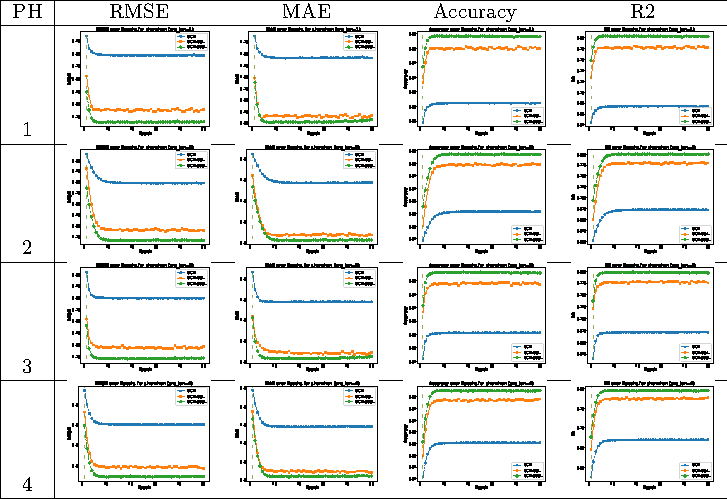
\includegraphics[width=\linewidth]{GCN_shenzhen_images_table-main.pdf}
  \caption{GCN training on SZ-taxi: GCN-cGSL (green) converges lower than standard GCN (blue).}
  \label{fig:gcn_shenzhen_performance}
\end{figure}

\begin{figure}[ht]
  \centering
  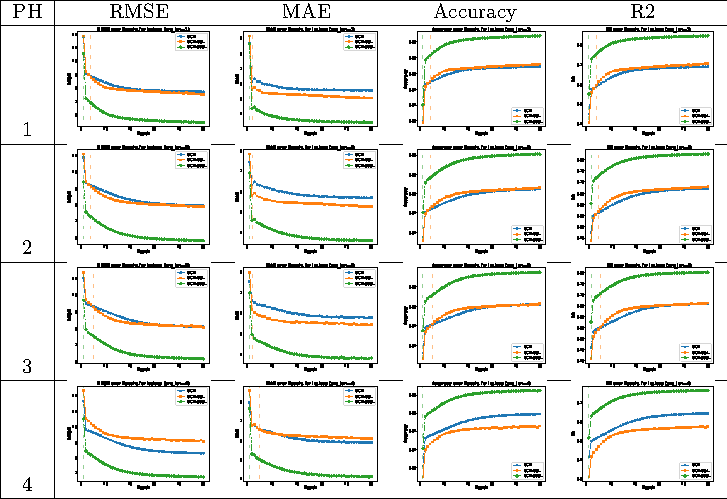
\includegraphics[width=\linewidth]{GCN_losloop_images_table-main.pdf}
  \caption{GCN training on Los-loop: GCN-cGSL (green) converges lower than standard GCN (blue).}
  \label{fig:gcn_losloop_performance}
\end{figure}

\begin{figure}[ht]
  \centering
  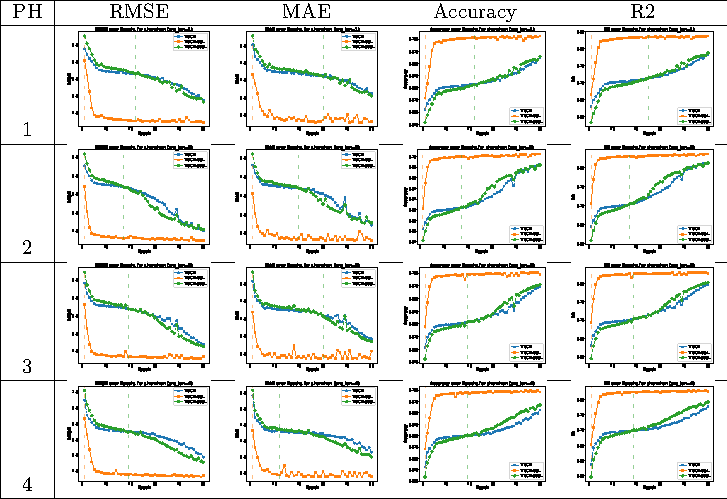
\includegraphics[width=\linewidth]{TGCN_shenzhen_images_table-main.pdf}
  \caption{TGCN training on SZ-taxi: TGCN-GSL (orange) converges lower than standard TGCN (blue).}
  \label{fig:tgcn_shenzhen_performance}
\end{figure}

\begin{figure}[ht]
  \centering
  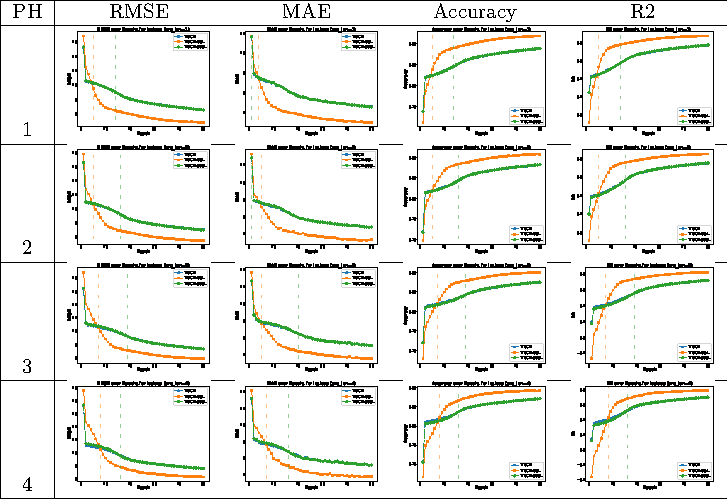
\includegraphics[width=\linewidth]{TGCN_losloop_images_table-main.pdf}
  \caption{TGCN training on Los-loop: TGCN-GSL (orange) converges lower than standard TGCN (blue).}
  \label{fig:tgcn_losloop_performance}
\end{figure}

% ============================================================
% APPENDIX: bibliometric
% ============================================================

\section{Bibliometric Analysis Methodology}\label{sec:Bibliometric-Methodology}

To justify the focus on graph-based approaches in traffic forecasting, we conducted a systematic bibliometric analysis.

\subsection{Data Collection}

A broad search in Scopus using ``traffic forecast*'' retrieved approximately 60,000 documents. Filtering for peer-reviewed English articles in Engineering or Computer Science yielded 784 articles (2000--2025).

\subsection{Keyword Processing}

The 6,343 unique keywords were reduced to 217 (frequency $\geq$ 10). Semantic clustering using Sentence-BERT embeddings grouped these into 66 meaningful concept clusters. Similar terms (e.g., ``graph neural network'', ``GNN'') were unified.

\subsection{Key Findings}

\begin{figure}[ht]
\centering
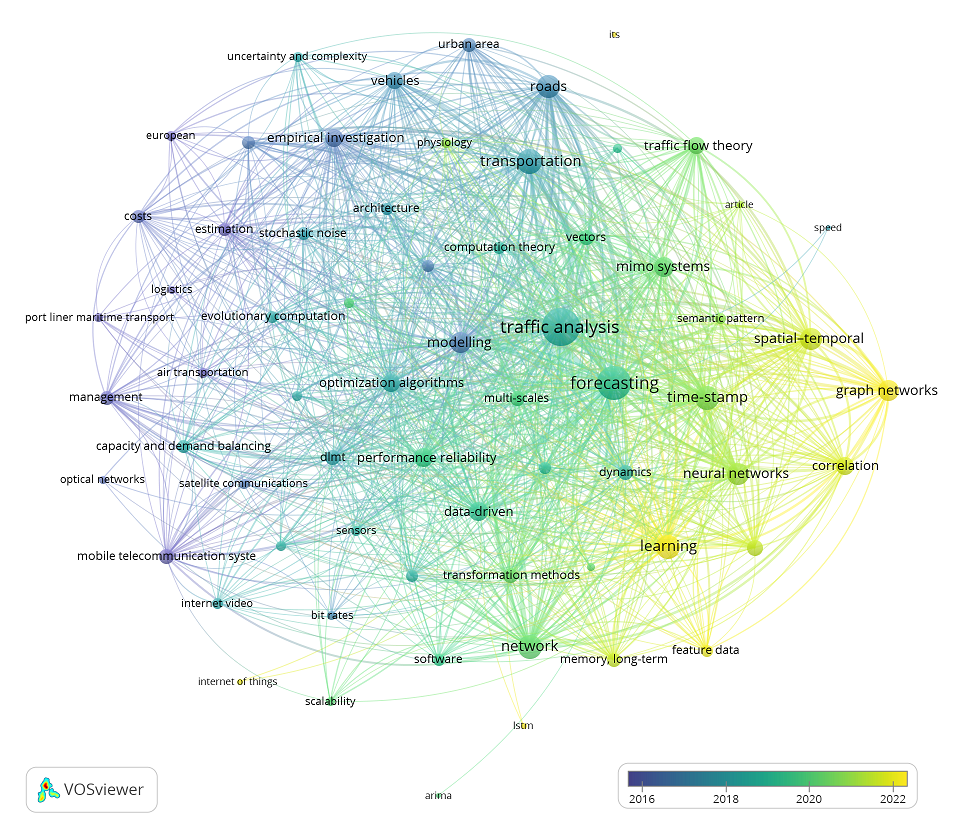
\includegraphics[width=0.9\linewidth]{scopus-clustered.png}
\caption{Clustered keyword co-occurrence network from 784 articles, colored by average publication year. Graph-based methods (right nodes) are the most recent focus.}
\label{fig:clustered_keywords}
\end{figure}

Figure~\ref{fig:clustered_keywords} reveals that graph-based methods have become the dominant recent methodological focus. However, nearly all rely on predefined graph structures---directly motivating our Graph Structure Learning approach.

\begin{figure}[ht]
\centering
\begin{subfigure}{0.32\textwidth}
    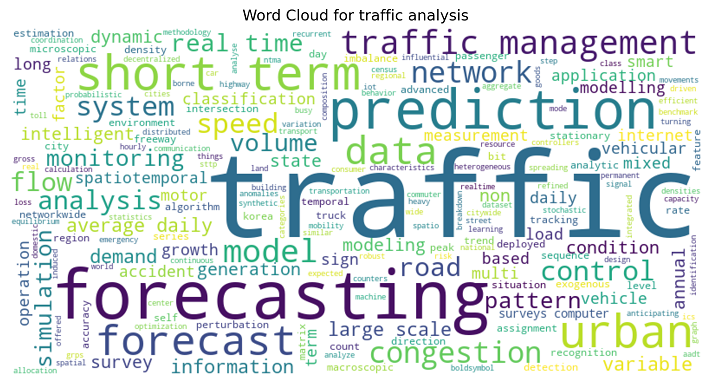
\includegraphics[width=\linewidth]{1-traffic analysis.png}
    \caption{Traffic Analysis}
\end{subfigure}
\hfill
\begin{subfigure}{0.32\textwidth}
    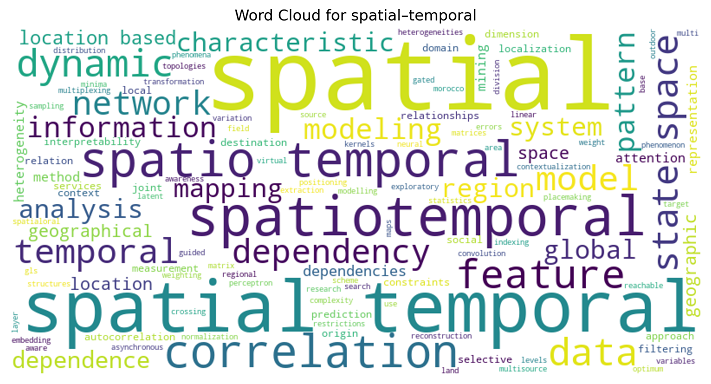
\includegraphics[width=\linewidth]{5-spatial–temporal.png}
    \caption{Spatio-Temporal}
\end{subfigure}
\hfill
\begin{subfigure}{0.32\textwidth}
    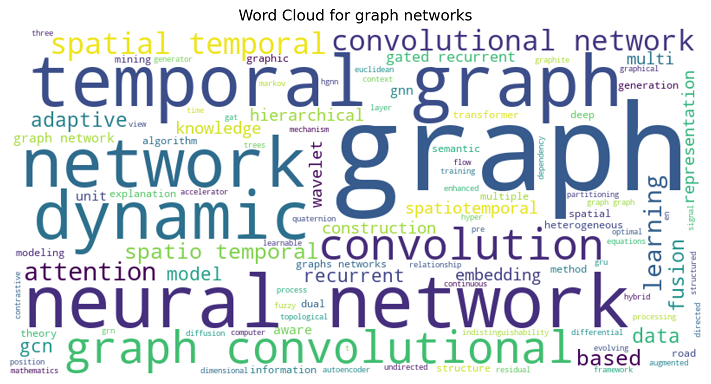
\includegraphics[width=\linewidth]{8-graph networks.png}
    \caption{Graph Networks}
\end{subfigure}
\caption{Word clouds from three key bibliometric clusters.}
\label{fig:word-clouds}
\end{figure}

% ============================================================
% APPENDIX: additional_diagnostics
% ============================================================

\section{Additional Diagnostics}\label{app:diagnostics}

\subsection{Graph Density Statistics}

Table~\ref{tab:density_stats} compares graph densities across methods.

\begin{table}[ht]
\centering
\caption{Graph density comparison (Los-loop, $N=207$).}
\label{tab:density_stats}
\begin{tabular}{lcc}
\toprule
\textbf{Graph} & \textbf{Edges} & \textbf{Density} \\
\midrule
Physical & 2833 & 0.0660 \\
NoGraph (identity) & 207 & 0.0048 \\
MultiGraph\_fixed ($\tau$=0.1) & 30 & 0.0007 \\
GatedMulti ($\tau$=0.1) & 30 & 0.0007 \\
\bottomrule
\end{tabular}
\end{table}

\subsection{SZ-Taxi Multi-Horizon Results}

Table~\ref{tab:sz_multiph} reports SZ-Taxi results, showing marginal GatedMulti improvement.

\begin{table}[ht]
\centering
\caption{SZ-Taxi multi-horizon results (seed=42). GatedMulti improvement is marginal.}
\label{tab:sz_multiph}
\begin{tabular}{lcccc}
\toprule
\textbf{Method} & \textbf{PH=1} & \textbf{PH=2} & \textbf{PH=3} & \textbf{PH=4} \\
\midrule
NoGraph & 4.116 & 4.160 & 4.189 & 4.221 \\
\textbf{GatedMulti} & 4.108 & 4.149 & 4.184 & 4.221 \\
\bottomrule
\end{tabular}
\end{table}

\subsection{DAGMA Computational Cost}

Multi-lag DAGMA runtime on standard hardware (RTX 3090):
\begin{itemize}
    \item SZ-Taxi ($624 \times 624$): approximately 100 minutes per prediction horizon
    \item Los-loop ($828 \times 828$): approximately 240 minutes per prediction horizon
\end{itemize}
Total computation for all 8 DAGMA runs (2 datasets $\times$ 4 PHs): approximately 28 hours.

\end{appendices}

\bibliography{MyReferences}

\end{document}
